\chapter{Background}
\label{ch:background}

%%%%%%%%%%%%%%%%%%%%%%%%%%%%%%%%%%%%%%%%%%%%%%%%%
% ANOMALY DETECTION
%%%%%%%%%%%%%%%%%%%%%%%%%%%%%%%%%%%%%%%%%%%%%%%%%
\section{Anomaly detection}
\newglossaryentry{anomaly}{
    name=anomaly,
    plural=anomalies,
    description={patterns in data that do not conform to a well defined notion 
                 of normal behavior}
}
Anomaly detection is the process of detecting patterns in a given data set that 
do not conform to an established normal behavior \cite{CHANDOLA07}.

The importance of anomaly detection is due to the fact that anomalies in data
translate to significant (and often critical) actionable information in a wide 
variety of application domains \cite{CHANDOLA07}.

% WHAT ARE ANOMALIES?
\subsection{What are anomalies?}
\index{anomaly}
\Gls{anomaly} are patterns in data that do not conform to a well defined notion 
of normal behavior. Figure~\ref{fig:2d-anomalies} illustrates anomalies in a 
simple 2-dimensional data set. The data has two normal regions, $N_{1}$ and 
$N_{2}$, since most observations lie in these two regions. Points that are 
sufficiently far away from the regions, such as points $o_{1}$ and $o_{2}$, and 
points in region $O_{3}$, are anomalies.

\begin{figure}[H]
\centering
\ifpdf
	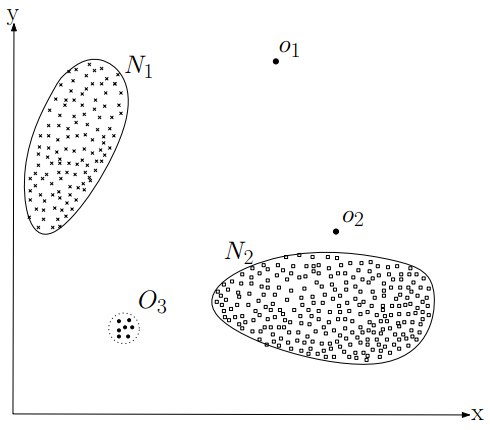
\includegraphics[width=0.5\textwidth]{2d-anomalies.png}
\else
	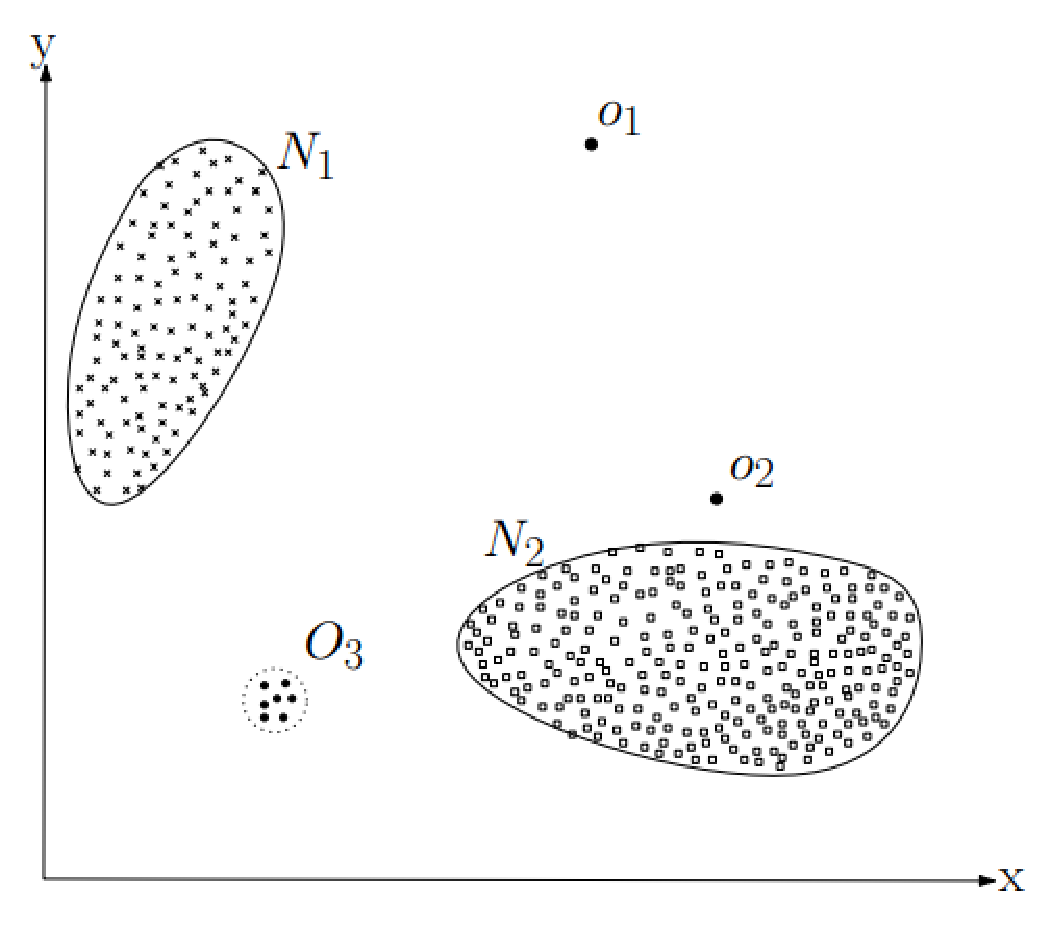
\includegraphics[width=0.5\textwidth]{2d-anomalies.eps}
\fi
\caption{A simple example of anomalies in a 2-dimensional data set.}
\label{fig:2d-anomalies}
\end{figure}

% CHALLENGES
\subsection{Challenges}
At an abstract level, an anomaly is defined as a pattern that does not conform 
to expected normal behavior. A straightforward anomaly detection approach, 
therefore, is to define a region representing normal behavior and declare any 
observation in the data which does not belong to this normal region as an 
anomaly. But several factors make this apparently simple approach very 
challenging:
\begin{itemize}
\item Defining a normal region which encompasses every possible normal behavior 
is very difficult. In addition, the boundary between normal and anomalous 
behaviour is often not precise. Thus an anomalous observation which lies close
to the boundary can actually be normal, and vice-versa.
\item When anomalies are the result of malicious actions, the malicious 
adversaries often adapt themselves to make the anomalous observations appear 
like normal, thereby making the task of defining normal behavior more difficult.
\item In many domains normal behavior keeps evolving and a current notion of
normal behavior might not be su±ciently representative in the future.
\item The exact notion of an anomaly is different for different application 
domains. For example, in the medical domain a small deviation from normal (for
example, fluctuations in body temperature) might be an anomaly, while similar 
deviation in the stock market domain (for example, fluctuations in the value of 
a stock) might be considered as normal. Thus applying a technique developed in 
one domain to another is not straightforward.
\item Availability of labeled data for training/validation of models used by 
anomaly detection techniques is usually a major issue.
\item Often the data contains noise which tends to be similar to the actual 
anomalies and hence is di±cult to distinguish and remove.
\end{itemize}

Due to the above challenges, the anomaly detection problem, in its most general
form, is not easy to solve. In fact, most of the existing anomaly detection 
techniques solve a specific formulation of the problem. The formulation is 
induced by various factors such as nature of the data, availability of labeled 
data, type of anomalies to be detected, etc. Often, these factors are determined
by the application domain in which the anomalies need to be detected. 
Researchers have adopted concepts from diverse disciplines such as statistics, 
machine learning, data mining, information theory, spectral theory, and have 
applied them to specific problem formulations.

%%%%%%%%%%%%%%%%%%%%%%%%%%%%%%%%%%%%%%%%%%%%%%%%%
% RANDOM PROJECTIONS
%%%%%%%%%%%%%%%%%%%%%%%%%%%%%%%%%%%%%%%%%%%%%%%%%
\section{Random projections}

%%%%%%%%%%%%%%%%%%%%%%%%%%%%%%%%%%%%%%%%%%%%%%%%%
% DISTANCE METRICS
%%%%%%%%%%%%%%%%%%%%%%%%%%%%%%%%%%%%%%%%%%%%%%%%%
\section{Distance metrics}
\index{distance,metric}
\newglossaryentry{distance}{
    name=distance,
    description={a quantitative description of how far apart three objects are}
}
\newglossaryentry{metric}{
    name=metric,
    description={a function describing how close or far away data points in some 
                 space are from each other}
}
\gls{distance} is a quantitative description of how far apart two objects are. 
Mathematically, a \gls{distance} or \gls{metric} is a function describing how 
close or far away data points in some space are from each other \cite{KHOA12}.

% EUCLIDEAN DISTANCE
\subsection{Euclidean distance}

% MAHALANOBIS DISTANCE
\subsection{Mahalanobis distance}

% GRAPH GEODESIC DISTANCE
\subsection{Graph geodesic distance}

%%%%%%%%%%%%%%%%%%%%%%%%%%%%%%%%%%%%%%%%%%%%%%%%%
% NEAREST NEIGHBOUR ALGORITHMS
%%%%%%%%%%%%%%%%%%%%%%%%%%%%%%%%%%%%%%%%%%%%%%%%%
\section{Nearest Neighbour Algorithms}

%%%%%%%%%%%%%%%%%%%%%%%%%%%%%%%%%%%%%%%%%%%%%%%%%
% MATRICES
%%%%%%%%%%%%%%%%%%%%%%%%%%%%%%%%%%%%%%%%%%%%%%%%%
\section{Matrices}

% EIGENVECTORS AND EIGENVALUES
\subsection{Eigenvectors and Eigenvalues}
This section will briefly recall some basic definitions of eigenvectors and
eigenvalues, as well as some of their basic properties.

A vector $\mathbf{v}$ is an eigenvector of a matrix $M$ of eigenvalue $\lambda$ 
if:
\begin{displaymath}
M\mathbf{v} = \lambda\textbf{v}
\end{displaymath}

If $\mathbf{v_{1}}$ is an eigenvector of M of eigenvalue $\lambda_{1}$, 
$\mathbf{v_{2}}$ is an eigenvector of M of eigenvalue $\lambda_{2} \neq 
\lambda_{1}$, and $M$ is symmetric, then $\mathbf{v_{1}}$ is orthogonal to 
$\mathbf{v_{2}}$.

For a symmetric matrix $M$, the multiplicity of an eigenvalue $\lambda$ is the
dimension of the space of eigenvectors of eigenvalue $\lambda$. Also recall that
every $n{\times}n$ symmetric matrix has $n$ eigenvalues, counted with 
multiplicity. Thus, it has an orthonormal basis of eigenvectors, 
$\begin{Bmatrix} \mathbf{v_{1}} & \ldots & \mathbf{v_{n}} \end{Bmatrix}$ with
eigenvalues $\lambda_{1} \leq \lambda_{2} \leq \ldots \leq \lambda_{n}$ so that:
\begin{displaymath}
M\mathbf{v_{i}} = \lambda_{i}\mathbf{v_{i}} \quad \forall i
\end{displaymath}

If we let $V$ be the matrix whose $i$th column is $v_{i}$ and $\Lambda$ be the 
diagonal matrix whose $i$th diagonal is $\lambda_{i}$, we can write this more 
compactly as:
\begin{displaymath}
MV = V\Lambda
\end{displaymath}

Multiplying by $V^{T}$ on the right, we obtain the eigen-decompisition of $M$:
\begin{displaymath}
M = MVV^{T} = V{\Lambda}V^{T} = \sum_{i} \lambda_{i}\mathbf{v_{i}}\mathbf{v_{i}^{T}}
\end{displaymath}

% LAPLACIAN MATRICES
\subsection{Laplacian Matrices}
\nocite{BERKEYLEY99}
\nocite{PATI11}
\nocite{SPIELMAN09}
\newglossaryentry{LaplacianMatrix}{
    name={Laplacian Matrix},
    plural={Laplacian Matrices},
    description={a matrix representation of a graph}
}
Recall that a weighted, undirected graph $G = (V,E,w)$ is essentially an 
undirected graph $G = (V,E)$ along with a function $w : E \rightarrow 
\Re^{+}$, where $\Re^{+}$ denotes the set of positive real numbers.

The adjacency matrix of a weighted graph $G$ will be denoted $A_{G}$, and is
given by:
\begin{displaymath}
A_{G}(i,j) := 
    \left\{
        \begin{array}{ll}
            \mathit{w}(i,j) &   \quad \text{if $(i,j) \in E$} \\
            0 &                 \quad \text{otherwise}
        \end{array}
    \right.
\end{displaymath}

The degree matrix of a weighted graph $G$ will be denoted $D_{G}$, and is the
diagonal matrix such that:
\begin{displaymath}
D_{G}(i,i) = \sum_{j} A_{G}(i,j)
\end{displaymath}

A \gls{LaplacianMatrix} is a matrix representation of a graph, defined by the
equation:
\begin{displaymath}
L_{G} = D_{G} - A_{G}
\end{displaymath}

Now, let $G_{1,2}$ be a graph on two vertices with a single edge of weight $1$.
\begin{displaymath}
L_{G_{1,2}} :=
    \begin{bmatrix}
        1 & -1 \\
        -1 & 1
    \end{bmatrix}
\end{displaymath}

For the graph with $n$ vertices and just one edge between vertices $u$ and $v$, 
we can define the \gls{LaplacianMatrix} similarly. For concreteness, I'll call 
this graph $G_{u,v}$. It's \gls{LaplacianMatrix} is the $n{\times}n$ matrix 
whose only non-zero entries are in the intersections of rows and columns $u$ and
$v$. The $2{\times}2$ matrix at the intersections of these rows and columns is, 
of course:
\begin{displaymath}
    \begin{bmatrix}
        1 & -1 \\
        -1 & 1
    \end{bmatrix}
\end{displaymath}

For a weighted graph $G = (V,E,w)$, we define:
\begin{displaymath}
L_{G} := \sum_{(u,v) \in E} w(u,v)L_{G_{u,v}}
\end{displaymath}

\paragraph{Properties}
For a graph $G$ and its \gls{LaplacianMatrix} $L$ with eigenvalues 
$\lambda_{0} < \lambda_{1} < \ldots < \lambda_{n-1}$:

\begin{itemize}
\item $L$ is a symmetric matrix. This means the eigenvalues of $L$ are real, and
its eigenvectors are real and orthogonal.
\item $L$ is always positive-semidefinite ($\forall i, \lambda_{i} \geq 0; 
\lambda_{0} = 0$).
\item Let $G = (V,E)$ be a graph, and let $0 = \lambda_{1} \leq \lambda_{2}
\leq \ldots \leq \lambda_{n}$ be the eigenvalues of its Laplacian Matrix. Then, 
$\lambda_{2} > 0$ if and only if $G$ is connected.
\item The number of times $0$ appears as an eigenvalue in the Laplacian Matrix 
is the number of connected components in the graph.
\item $\lambda_{0}$ is always $0$ because every \gls{LaplacianMatrix} has an 
eigenvector of $\begin{bmatrix} 1 & 1 & \ldots & 1 \end{bmatrix}$ that, for each
row, adds the corresponding node's degree to a ``-1'' for each neighbour, 
thereby producing zero by definition.
\item The smallest non-zero eigenvalue of $L$ is called the spectral gap.
\item If we arbitarily assign an orientation to the edges in $G$ and label each
edge, then we can define the vertex edge incidence matrix $Q$ by:
\begin{displaymath}
Q_{ij} := 
    \left\{
        \begin{array}{ll}
            1 &     \quad \text{if $e_{j}$ starts from $i$} \\
            -1 &    \quad \text{if $e_{j}$ ends at $i$} \\
            0 &     \quad \text{otherwise}
        \end{array}
    \right.
\end{displaymath}
Then the \gls{LaplacianMatrix} $L$ satisfies $L = Q^{T}Q$, regardless of the 
orientation of the edges.
\item The second smallest eigenvalue of $L$ ($\lambda_{2}$) is the algebraic 
connectivity of $G$. $\lambda_{2} > 0$ if and only if $G$ is connected.
\end{itemize}

%%%%%%%%%%%%%%%%%%%%%%%%%%%%%%%%%%%%%%%%%%%%%%%%%
% COMMUTE TIME
%%%%%%%%%%%%%%%%%%%%%%%%%%%%%%%%%%%%%%%%%%%%%%%%%
\section{Commute Time}

% ANOMALY DETECTION USING COMMUTE TIME
\subsection{Anomaly Detection Using Commute Time}

%%%%%%%%%%%%%%%%%%%%%%%%%%%%%%%%%%%%%%%%%%%%%%%%%
% SOLVERS
%%%%%%%%%%%%%%%%%%%%%%%%%%%%%%%%%%%%%%%%%%%%%%%%%
\section{Solvers}

% SPIELMAN-TENG SOLVER
\subsection{Spielman-Teng Solver}
\nocite{SPIELMANTANG09}
Spielman and Teng presented a randomised algorithm that, on input a symmetric, 
weakly diagonally dominant $n{\times}x$ matrix $A$ with $m$ non-zero entries and
an $n$-vector $\mathbf{b}$, produces an $\tilde{\mathbf{x}}$ such that 
$\begin{Vmatrix} \tilde{\textbf{x}} - A^{\dagger}\textbf{b} \end{Vmatrix}_{A} 
\leq \epsilon \begin{Vmatrix} A^{\dagger}\mathbf{b} \end{Vmatrix}_{A}$ in 
expected time:
\begin{displaymath}
m \log^{O(1)} n \log (1/\epsilon)
\end{displaymath}
